\documentclass{article}


% if you need to pass options to natbib, use, e.g.:
%     \PassOptionsToPackage{numbers, compress}{natbib}
% before loading neurips_2024


% ready for submission
\usepackage{neurips_2024}


% to compile a preprint version, e.g., for submission to arXiv, add add the
% [preprint] option:
%     \usepackage[preprint]{neurips_2024}


% to compile a camera-ready version, add the [final] option, e.g.:
%     \usepackage[final]{neurips_2024}


% to avoid loading the natbib package, add option nonatbib:
%    \usepackage[nonatbib]{neurips_2024}


\usepackage[utf8]{inputenc} % allow utf-8 input
\usepackage[T1]{fontenc}    % use 8-bit T1 fonts
\usepackage{hyperref}       % hyperlinks
\usepackage{url}            % simple URL typesetting
\usepackage{booktabs}       % professional-quality tables
\usepackage{amsfonts}       % blackboard math symbols
\usepackage{nicefrac}       % compact symbols for 1/2, etc.
\usepackage{microtype}      % microtypography
\usepackage{xcolor}         % colors

% Packages added by me.
\usepackage{amsmath}
\usepackage{amssymb}
\usepackage{amsthm}
\usepackage{todonotes}
\usepackage{bm}
\usepackage{subcaption}
\usepackage[ruled]{algorithm2e}

\def\ci{\perp\!\!\!\!\!\perp}

\newtheorem{definition}{Definition}
\newtheorem{proposition}{Proposition}

\title{Title}


% The \author macro works with any number of authors. There are two commands
% used to separate the names and addresses of multiple authors: \And and \AND.
%
% Using \And between authors leaves it to LaTeX to determine where to break the
% lines. Using \AND forces a line break at that point. So, if LaTeX puts 3 of 4
% authors names on the first line, and the last on the second line, try using
% \AND instead of \And before the third author name.


\author{%
  David S.~Hippocampus\thanks{Use footnote for providing further information
    about author (webpage, alternative address)---\emph{not} for acknowledging
    funding agencies.} \\
  Department of Computer Science\\
  Cranberry-Lemon University\\
  Pittsburgh, PA 15213 \\
  \texttt{hippo@cs.cranberry-lemon.edu} \\
  % examples of more authors
  % \And
  % Coauthor \\
  % Affiliation \\
  % Address \\
  % \texttt{email} \\
  % \AND
  % Coauthor \\
  % Affiliation \\
  % Address \\
  % \texttt{email} \\
  % \And
  % Coauthor \\
  % Affiliation \\
  % Address \\
  % \texttt{email} \\
  % \And
  % Coauthor \\
  % Affiliation \\
  % Address \\
  % \texttt{email} \\
}

\begin{document}

\maketitle

\begin{abstract}
	The initial step in a causal analysis involves determining the causal
	structure between the variables from data typically in the form of a
	Directed Acyclic Graph (DAG) or an Structural Equation Model (SEM).
	This procedure, known as \emph{causal discovery}, has been extensively
	studied for both DAGs and SEMs. While numerous automated algorithms
	exist for estimating DAGs from datasets, their application in applied
	fields remain limited, possibly due to a lack of confidence in these
	algorithms stemming from them making obvious mistakes, and the
	difficulties in choosing the right algorithm for a given dataset. As a
	result, in applied disciplines, DAGs are predominantly constructed
	manually based on domain expertise making it vital to test the fit of
	these models to the data and potentially modifying them to improve the
	fit. Conversely, SEMs are typically constructed manually where
	researchers come up with an initial model based on domain knowledge and
	then iteratively assess its fit and modify the model according to that.
	This process is commonly known as \emph{specification search} where
	expert knowledge combined with data-driven methods like
	\emph{modification indices} is used to guide the modification process.
	In the case of DAGs, although statistical tests are available that can
	assess the fit of the model, there are no methods that can guide our
	modification process to improve the fit.

	Inspired by the modification process in SEMs, in this paper, we
	introduce a data-driven modification process aimed at assisting
	researchers in manually constructing or modifying DAGs generated by an
	algorithm. The first step of this process involves identifying pairs of
	variables whose observed association is not fully explained by the
	model. The user can then make modifications to the model by adding
	edges between such variables while using their domain expertise to
	decide the direction of the edge. For the measure of association, in
	the case of continuous and discrete variables we can use effect sizes,
	however no such measure of association is present for mixed data. We
	propose a novel (conditional) measure of association for mixed data
	based on canonical correlations. We also present a graphical web-tool
	that can assist researchers in iteratively modifying and constructing
	their DAGs. We theoretically show that in the presence of an oracle,
	this iterative modification process is consistent in recovering the
	true DAG. Empirically, we show that this process performs comparably to
	PC and Hill-Climb Search algorithms if the user is able to correctly
	identify the direction of the edge in one out of three cases.
\end{abstract}

\section{Introduction}

To perform any causal effect identification or estimation in Pearl's Directed
Acyclic Graphs (DAGs) based causal framework usually requires to come up with
the DAG structure. Learning these DAG structures from data is known as
\emph{causal discovery}. Plenty of algorithms have been developed for these in
the literature such as constraint-based methods such as PC, FCI, score based
methods such as Hill-Climb Search, GES, and constrained continuous optimization
based such as No TEARS. All these algorithms take different approaches to
causal discovery, constraint-based algorithms utilize statistical conditional
independence (CI) tests to come up with a model structure, the score-based
methods iteratively perform local modifications to the model such that some
score function is maximized, the continuous optimization methods reformulate
the problem statement as a constrained optimization problem and use
optimization algorithms to come up with a graph.

Even though we have various algorithms for doing casual discovery, yet
researchers in applied fields prefer to construct these DAGs manually based on
their domain knowledge. We hypothesize the following two reasons for low
adaption of these methods in applied sciences:

\begin{enumerate}
	\item Biased towards sparse graphs.
	\item Algorithms making obvious mistakes: These algorithms often make
		very obvious mistakes, making it harder for the user to trust
		them.
	\item Difficulties in choosing an algorithm: For any given dataset, the
		user need to make a choice of the algorithm. Given that these
		algorithms work very differently, it can be difficult to make a
		choice. Additionally, each of these algorithms have
		hyperparameters and choices to make for them, making it
		difficult. As there is no way to evaluate the performance of
		these algorithms on our dataset.
\end{enumerate}

Both in the cases when the DAG is an output of an algorithm or when constructed
by hand, it is vital to test these models against data before using them for
making any inference. 

In the field of Structural Equation Models (SEMs), models are typically
constructed by hand. Researchers typically come up with an initial model, which
then they use the data to make modifications to. This process is known as
\emph{Specification Search}. One of the common ways to do this is through
\emph{modification indices} where a global fit of the model is measured with
different modification to the model. Utilizing expert knowledge to select the
appropriate modification that gives the maximum improvement to the global fit.

In the case of DAGs however, we do not have any way to As these CI based
testing uses p-values and effect size measures from CI tests for testing. And
as mixed data is common, we need both a test and effect size measure for mixed
data. Recently, a few CI tests for mixed data have been proposed but an effect
size is still missing.

\begin{enumerate}
	\item We present a procedure to construct and modify DAGs using domain
		knowledge.
	\item The presented procedure uses a (conditional) measure of
		association between variables. In the simple case of continuous
		or discrete variables, effect size measures can be used,
		however as no such measure exists for mixed data, we present
		one.
	\item Lastly, to assist researchers in using the DAG construction
		approach, we developed a web-based tool to help researches in
		constructing and modifying their DAGs.
\end{enumerate}

\begin{figure}
		\centering
		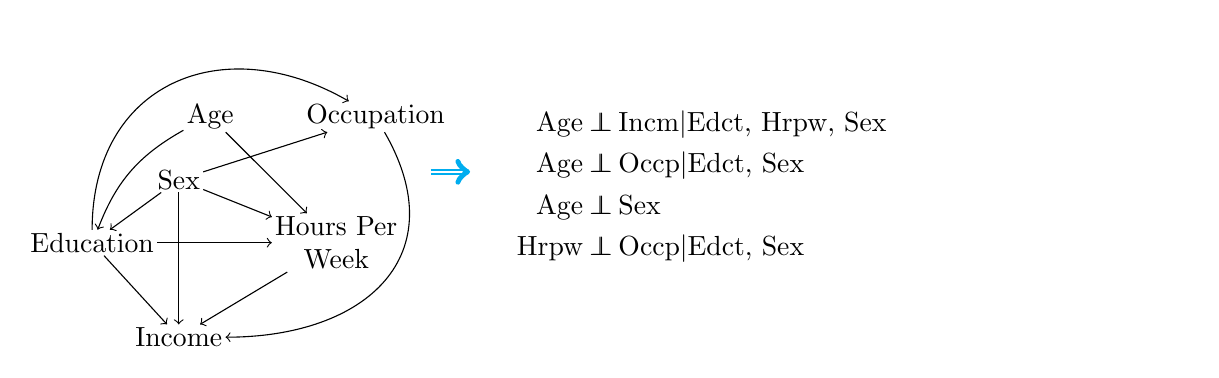
\begin{tikzpicture}
			\begin{scope}[yshift=0.7cm, scale=1]
			\tikzstyle{every node}=[align=center, inner sep=1pt]
				\node (sex) at (-0.7, -0.8) {Sex};
				\node (age) at (-0.3, 0) {Age};
				\node (ed) at (-1.8, -1.6) {Education};
				\node (occ) at (1.8, 0) {Occupation};
				\node (hrpw) at (1.3, -1.6) {Hours Per \\ Week};
				\node (income) at (-0.7, -2.8) {Income};
			
				\draw[->]  (age) to[bend right=20] (ed);
				\draw[->]  (sex) to (ed);
				\draw[->]  (age) to (hrpw);
				\draw[->]  (ed) to (hrpw);
				\draw[->]  (sex) to (hrpw);
				\draw[->]  (ed) to (income);
				\draw[->]  (hrpw) to (income);
				\draw[->]  (occ) to[out=300, in=0, looseness=1.4] (income.east);
				\draw[->]  (sex) to (income);
				\draw[->]  (ed) to[out=90, in=150, looseness=1.3] (occ);
				\draw[->]  (sex) to (occ);	
			\end{scope}
			\draw[thick, ->, double, cyan] (2.5,0) -- (3,0);
			\node[rectangle, align=center, inner sep=1pt] at (6, 0) {
				\begin{minipage}{\textwidth}
					\begin{equation*}
						\begin{split}
							\textnormal{Age} &\ci \textnormal{Incm} \rvert \textnormal{Edct, Hrpw, Sex} \\
							\textnormal{Age} &\ci \textnormal{Occp} \rvert \textnormal{Edct, Sex} \\
							\textnormal{Age} &\ci \textnormal{Sex} \\
							\textnormal{Hrpw} &\ci \textnormal{Occp} \rvert \textnormal{Edct, Sex} \\
						\end{split}
					\end{equation*}
				\end{minipage}
				};
		\end{tikzpicture}
		\caption{\todo[inline]{Show a full example of testing using this model}}
\end{figure}


\section{Background}
We represent uni-dimensional variables as $ X $ and multi-dimensional variables
as $ \bm{Z} $. We consider the case of estimating association between $ X $,
and $ Y $ is the presence of a set of conditioning variables $ \bm{Z} = Z_1,
\cdots, Z_k $, potentially being an empty set $ \bm{Z} = \emptyset $. We use $
\rvert \bm{Z} \rvert $ to denote the cardinality of the variable $ \bm{Z} $. We
consider various scenarios where the variables $ X $, $ Y $ and $ \bm{Z} $
could be either discrete, ordinal, or continuous. With mixed data, we mean an
arbitrary mix of variable types among $ X $, $ Y $, and $ \bm{Z} $.

We consider the problem of estimating the partial (or conditional) association
between $ X $ and $ Y $ in the presence of the conditioning set $ Z $. When $ Z
= \emptyset $, this is equivalent to the marginal association between $ X $ and
$ Y $.

\todo[inline]{Add more notation as they come}

\subsection{Effect size Measures}
In this section, we give a background on some of the commonly used effect size
measures in the context of CI testing.

\paragraph{$ X $ and $ Y $ are continuous}
In the case when $ \bm{Z} = \emptyset $, and when both $ X $ and $ Y $ are
continuous variables, Pearson's correlation coefficient based test can be used
which also gives an effect size measure. The p-value computation requires the
data to be normally distributed but other statistics can be used such as
Spearman's rank correlation, or Kendall's Tau.

In the case when $ \bm{Z} \neq \emptyset $, then partial correlations can be used.
In this case we first compute the residuals of $ X $ and $ Y $ using $ \bm{Z} $ as 
the predictor. We start by training two model $ X \sim \bm{Z} $ and $ Y \sim \bm{Z} $.
Then the residuals are computed for both as $ R_X = X - \hat{X} $ and $ R_Y = Y - \hat{Y} $.
After this we can do a normal non-conditional test on $ R_X $ and $ R_Y $.

\paragraph{All variables are discrete}

When $ \bm{Z} = \emptyset $, in the case of discrete variables, chi-squared test can be used. Effect size 
measures such as Cram\'er's V are available for it.

When $ \bm{Z} \neq \emptyset $, we can do stratification.


\paragraph{$ X $ is ordinal and $ Y $ is continuous}
Polyserial Correlation

When $ \bm{Z} = \emptyset $, ordinal variable can be assumed to be coming from a thresholded normal distribution, estimate the thresholds and latent variable to compute 
the correlation coefficient.

\paragraph{$ X $ and $ Y $ are ordinal}
Polychoric Correlation

\paragraph{Mixed data}
Recently multiple tests for mixed data have been proposed but they do not have
an effect size measure. We propose one based on canonical correlations.

\subsection{Canonical Correlation}
Canonical correlations are generalization of correlations to multi-dimensional variables.

\begin{definition}
	Given two sets of random variables $ \bm{U} = (U_1, U_2, \cdots, U_p) $
	and $ \bm{V} = (V_1, V_2, \cdots, V_q) $, canonical correlation between
	them, $\rho(\bm{U}, \bm{V}) $ is defined as:
		
	\begin{equation}
		\rho(\bm{U}, \bm{V}) = \sup_{a, b} \frac{a^T \Sigma_{\bm{U}\bm{V}} b}{\sqrt{a^T \Sigma_{\bm{U}\bm{U}} a} \sqrt{b^T \Sigma_{\bm{V}\bm{V}} b}}
	\end{equation}

\end{definition}
	
	Canonical correlations try to find linear transformations $ a $ and $ b
	$ of $ \bm{U} $ and $ \bm{V} $ such that the correlations between the
	columns of $ a^T \bm{U} $ and $ b^T \bm{V} $ is maximized. The
	individual columns of $ a^T \bm{U} $ and $ b^T \bm{V} $ are
	independent. In the case when $ \rvert U \rvert = \rvert V \rvert = 1$,
	canonical correlations are equivalent to Pearson's correlation
	coefficient.

Multiple effect sizes measures based on canonical correlation are available.
\begin{itemize}
	\item Wilks' Lambda: $ \Lambda = \prod (1 - \phi_i^2) $
	\item Roy's Largest Root: $ \theta = \phi_{\max}^2 $
	\item Pillai's Trace: $ \tau = \sum \phi_i^2 $
\end{itemize}
We use Pillai's Trace in this paper. \todo[inline]{Why?}.

\section{Effect size for mixed data}
In this section, we use canonical correlations to define an effect size measure
for mixed data CI tests. Our approach is similar to the approach used for the
continuous variable case. 

\subsection{No conditional variables}
When we have no conditonal variables, we need to convert the variables into 

\subsection{Conditional Case}

\subsection{Connection to special cases}

\section{Web Tool}
As most of the DAGs in practice are built manually, we use our mixed data effect size measure to build a web-tool that aids researches in building DAGs.

% \begin{figure}
% 	\centering
% 	\begin{subfigure}{0.5\textwidth}
% 		\includegraphics[scale=0.25]{../../presentations/2024_05_das/2.png}
% 	\end{subfigure}%
% 	\begin{subfigure}{0.5\textwidth}
% 		\includegraphics[scale=0.25]{../../presentations/2024_05_das/5.png}
% 	\end{subfigure}
% 	\caption{Screenshots of the web-tool. \todo[inline]{Insert screenshots of the web-tool}}
% \end{figure}

\section{Empirical Analysis}
To compare how well does creating a graph manually based on effect sizes and
p-value compare to algorithmic approaches, we performed some empirical
analysis.

\subsection{Simulating an expert}
To simulate an expert building a model manually, we wrote a simple greedy simulation as shown in the Figure. The expert always starts with a graph with
no edges and chooses the pair of variables with the highest correlation between them. The expert based on some accuracy measure decides the direction
of the edge between these variables such that the new added edge does not create a cycle in the DAG.

\todo[inline]{Summarize this section and equation in an algorithm}
\todo[inline]{Show a consistency proof for this expert simulation}

\begin{equation}
	\begin{split}
		x &= \textnormal{rand}([0, 1]) \\
		O(\alpha) &= \begin{cases} 
			M \rightarrow Y, & \textnormal{if  } x <= \alpha \\
			\textnormal{rand}(M \rightarrow Y, M \leftarrow Y, None) & \textnormal{otherwise} \\
				\end{cases} \\
	\end{split}
\end{equation}

\begin{algorithm}
	\caption{Expert Simulation}
	\While{True}{
	   $ e \gets \textnormal{Effects}(G) > \textnormal{THRESHOLD} $\;
	   $ e \gets e - \textnormal{blacklist} $\;
	   \If {$ e = 0 $}{
		$ G \gets G - e $ \;
		$ \textnormal{blacklist} \gets \textnormal{blacklist} \cup e $\;
	   } \;
	   \If{$ \textnormal{len}(e) = 0$}{
		   $ \textnormal{return}(G) $\;
	   }
	   $ X, Y \gets \max_{X, Y} e $\;
	   $ dir \gets Expert(X, Y, \alpha) $\;
	   $ G \gets G \cup dir $\;
	}

\end{algorithm}

After adding each edge, we also check if the p-value of any existing edge shows independence. If that happens we remove that edge and blacklist that edge. 
Blacklisted edges are not suggested to the expert in future iterations. We repeat this till we have explained all the correlations in the dataset.

There is a possibility that this greedy expert gets stuck at incorrect graph structures as it does not do any backtracking to fix its earlier mistakes.


\subsection{Results}
\begin{figure}
	\begin{subfigure}{0.5\textwidth}
		\includegraphics{../code/plots/shd_ribbon.pdf}
	\end{subfigure}%
	\begin{subfigure}{0.5\textwidth}
		\includegraphics{../code/plots/sid_ribbon.pdf}
	\end{subfigure}
\end{figure}

\section{Conclusions}
\subsection{Using LLMs as experts}



\bibliographystyle{plain}
\bibliography{references.bib}

%%%%%%%%%%%%%%%%%%%%%%%%%%%%%%%%%%%%%%%%%%%%%%%%%%%%%%%%%%%%

\appendix

\section{Appendix / supplemental material}


Optionally include supplemental material (complete proofs, additional experiments and plots) in appendix.
All such materials \textbf{SHOULD be included in the main submission.}

%%%%%%%%%%%%%%%%%%%%%%%%%%%%%%%%%%%%%%%%%%%%%%%%%%%%%%%%%%%%

\include{checklist}

\end{document}
